\section{Performance evaluation}

We use the web service example described in the previous section, figure \ref{fig:fluxions}, to compare the fluxionnal execution model, to basic Javascript implementation, listing \ref{lst:classique}.
For this evaluation against the basic implementation, we developed different version of the fluxionnal execution models using different methods for chaining fluxions.

\begin{itemize}
	\item[\textbf{Chain}]
		This implementation chains fluxions one after another by a direct function call.
		It set the fluxions chain length maximum to the macimum function call stack size, and it make it impossible to interleave messages from network.

	\item[\textbf{NextTick}]
		This implementation uses the instruction \texttt{process.nextTick} to chain fluxions execution.
		This instruction makes it possible to probe network messages only every \textit{n} fluxions execution. By default \textit{n} is set to 1000.

	\item[\textbf{SetTimeout}]
		This implementation uses the instruction \texttt{setTimeout}.
		It probes network messages after every fluxion execution, thus networks messages can be interleaved between each local messages.
\end{itemize}

With these differents implementations, we want to highlight the advantages and drawbacks of the fluxionnal execution model.

\begin{figure}
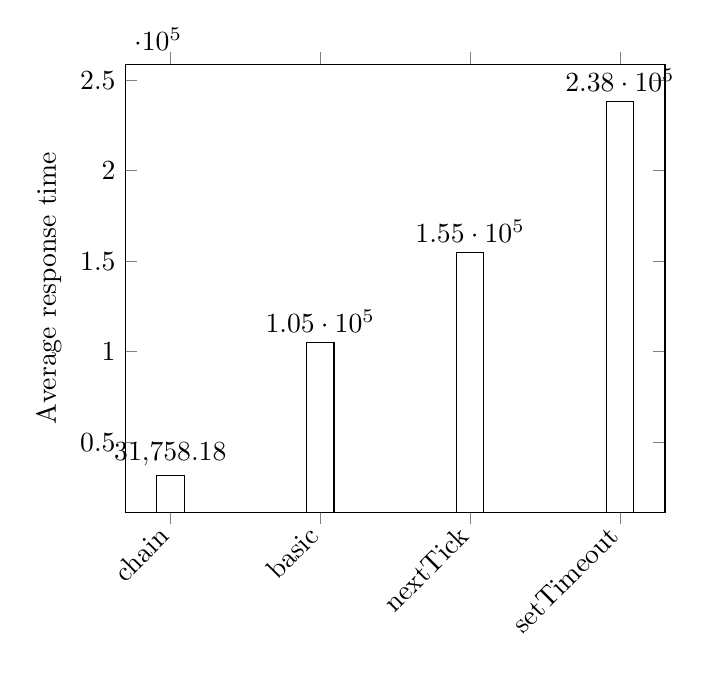
\begin{tikzpicture}
\begin{axis}[ybar, ylabel={Average response time}, nodes near coords, nodes near coords align={vertical}, xtick=data, x tick label style={rotate=45,anchor=east}, symbolic x coords={chain, basic, nextTick, setTimeout}]
\addplot[color=black]
coordinates {(chain,31758.1768)(basic,104941.1756)(nextTick,154836.3611)(setTimeout,238212.1012)};
\end{axis}
\end{tikzpicture}

\caption{Average response time for each implementation}
\label{fig:reponsetime}
\end{figure}

\begin{figure}
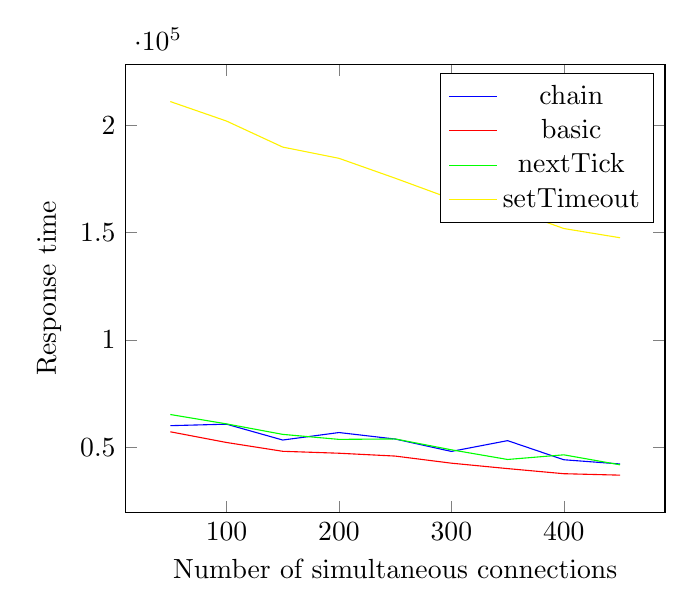
\begin{tikzpicture}
\begin{axis}[xlabel = Number of simultaneous connections, ylabel = Response time]
\addplot[color = blue] coordinates {(50, 60119.273172413814) (100, 60810.6431071428) (150, 53432.76434567901) (200, 56922.77901923074) (250, 53898.58569600001) (300, 48131.27358333333) (350, 53153.92239751554) (400, 44256.35740909089) (450, 42290.9475238095)};
\addplot[color = red] coordinates {(50, 57270.243655172475) (100, 52291.44685714285) (150, 48190.33730864198) (200, 47292.73021153844) (250, 45965.969983999996) (300, 42662.42051388889) (350, 40133.31911801241) (400, 37762.005920454554) (450, 37086.170052910056)};
\addplot[color = green] coordinates {(50, 65311.8316551724) (100, 60949.65357142856) (150, 56064.83629629629) (200, 53735.50407692306) (250, 53947.37227200004) (300, 48887.480125000024) (350, 44383.88242236024) (400, 46548.60027272731) (450, 41911.67969312167)};
\addplot[color = yellow] coordinates {(50, 210981.88593103446) (100, 201909.09617857132) (150, 189791.9731358024) (200, 184565.7975192309) (250, 175313.35167999993) (300, 165698.69973611107) (350, 161252.9545093167) (400, 151887.81970454537) (450, 147591.37962962966)};
\legend{chain, basic, nextTick, setTimeout};
\end{axis}
\end{tikzpicture}

\caption{Distribution of response time for each implementation}
\label{fig:distribution}
\end{figure}

\begin{figure}
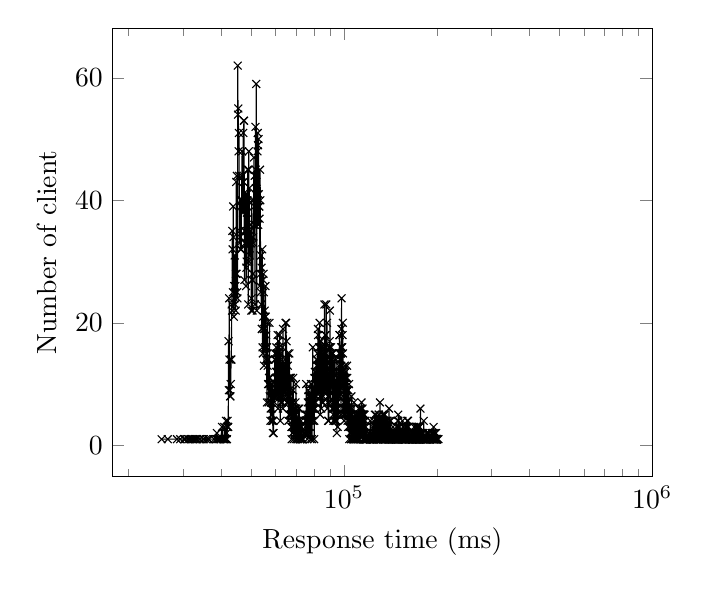
\begin{tikzpicture}
\begin{semilogxaxis}[xmin=0,xmax=1000000, ylabel=Number of client, xlabel=Response time (ms)]

\addplot[color=black, mark=x] coordinates {(25600,1)(26800,1)(28700,1)(29400,1)(30300,1)(30400,1)(30600,1)(31200,1)(31500,1)(31800,1)(32200,1)(32500,1)(32800,1)(33100,1)(33400,1)(34000,1)(34100,1)(34900,1)(35100,1)(35700,1)(36200,1)(36500,1)(37900,1)(38500,1)(38700,2)(38800,1)(39100,1)(39400,1)(39700,1)(39800,1)(40200,3)(40400,1)(40700,1)(40800,1)(40900,3)(41000,1)(41300,1)(41400,4)(41500,1)(41600,2)(41700,1)(41800,3)(41900,4)(42000,3)(42100,3)(42200,17)(42300,9)(42400,24)(42500,14)(42600,9)(42700,8)(42800,8)(42900,10)(43000,14)(43100,14)(43200,23)(43300,22)(43400,35)(43500,32)(43600,25)(43700,39)(43800,34)(43900,21)(44000,26)(44100,24)(44200,31)(44300,23)(44400,26)(44500,22)(44600,28)(44700,43)(44800,28)(44900,44)(45000,25)(45100,24)(45200,62)(45300,54)(45400,55)(45500,48)(45600,51)(45700,44)(45800,33)(45900,35)(46000,34)(46100,32)(46200,40)(46300,39)(46400,32)(46500,40)(46600,44)(46700,48)(46800,40)(46900,39)(47000,38)(47100,51)(47200,43)(47300,53)(47400,53)(47500,27)(47600,35)(47700,33)(47800,35)(47900,40)(48000,41)(48100,26)(48200,29)(48300,30)(48400,38)(48500,41)(48600,40)(48700,45)(48800,35)(48900,23)(49000,45)(49100,48)(49200,30)(49300,42)(49400,31)(49500,36)(49600,33)(49700,35)(49800,33)(49900,33)(50000,22)(50100,24)(50200,40)(50300,27)(50400,27)(50500,22)(50600,28)(50700,34)(50800,33)(50900,40)(51000,47)(51100,36)(51200,39)(51300,44)(51400,23)(51500,36)(51600,52)(51700,45)(51800,42)(51900,59)(52000,43)(52100,22)(52200,41)(52300,41)(52400,48)(52500,51)(52600,49)(52700,36)(52800,50)(52900,41)(53000,39)(53100,39)(53200,37)(53300,26)(53400,45)(53500,40)(53600,28)(53700,25)(53800,31)(53900,23)(54000,29)(54100,19)(54200,19)(54300,32)(54400,16)(54500,15)(54600,27)(54700,21)(54800,28)(54900,25)(55000,13)(55100,19)(55200,19)(55300,22)(55400,16)(55500,21)(55600,26)(55700,21)(55800,14)(55900,18)(56000,16)(56100,15)(56200,7)(56300,16)(56400,20)(56500,13)(56600,14)(56700,10)(56800,14)(56900,7)(57000,10)(57100,11)(57200,11)(57300,20)(57400,8)(57500,11)(57600,9)(57700,4)(57800,6)(57900,7)(58000,7)(58100,10)(58200,6)(58300,7)(58400,5)(58500,4)(58600,10)(58700,4)(58800,2)(58900,9)(59000,4)(59100,2)(59200,8)(59300,9)(59400,9)(59500,7)(59600,14)(59700,10)(59800,15)(59900,14)(60000,8)(60100,11)(60200,12)(60300,16)(60400,8)(60500,15)(60600,11)(60700,12)(60800,15)(60900,18)(61000,10)(61100,6)(61200,8)(61300,17)(61400,10)(61500,15)(61600,16)(61700,9)(61800,18)(61900,8)(62000,12)(62100,4)(62200,14)(62300,15)(62400,7)(62500,8)(62600,8)(62700,13)(62800,7)(62900,7)(63000,7)(63100,16)(63200,13)(63300,6)(63400,19)(63500,8)(63600,12)(63700,12)(63800,10)(63900,13)(64000,13)(64100,9)(64200,13)(64300,10)(64400,14)(64500,8)(64600,20)(64700,11)(64800,9)(64900,20)(65000,9)(65100,17)(65200,10)(65300,7)(65400,7)(65500,10)(65600,8)(65700,13)(65800,15)(65900,10)(66000,4)(66100,8)(66200,11)(66300,7)(66400,5)(66500,15)(66600,11)(66700,8)(66800,6)(66900,11)(67000,5)(67100,11)(67200,5)(67300,11)(67400,5)(67500,3)(67600,1)(67700,7)(67800,3)(67900,4)(68000,2)(68100,9)(68200,7)(68300,9)(68400,11)(68500,5)(68600,3)(68700,1)(68800,5)(68900,5)(69000,5)(69100,5)(69200,6)(69300,4)(69400,2)(69500,6)(69600,7)(69700,1)(69800,10)(69900,5)(70000,6)(70100,3)(70200,2)(70300,3)(70400,4)(70500,1)(70600,2)(70700,4)(70800,2)(70900,1)(71000,3)(71100,6)(71200,2)(71300,3)(71400,4)(71500,4)(71600,6)(71700,3)(71800,3)(72000,1)(72100,1)(72200,1)(72300,3)(72400,2)(72500,4)(72600,2)(72700,2)(72800,1)(72900,3)(73000,1)(73200,1)(73600,1)(73700,1)(74200,2)(74300,2)(74400,2)(74700,2)(74900,3)(75000,4)(75100,5)(75200,4)(75300,4)(75400,10)(75500,2)(75600,4)(75700,4)(75800,5)(75900,3)(76000,1)(76100,2)(76200,2)(76300,7)(76400,3)(76500,3)(76600,9)(76700,5)(76800,8)(76900,5)(77000,8)(77100,7)(77200,8)(77300,2)(77400,3)(77500,5)(77600,8)(77700,6)(77800,1)(77900,4)(78000,4)(78100,10)(78200,8)(78300,8)(78400,10)(78500,8)(78600,6)(78700,1)(78800,5)(78900,7)(79000,6)(79100,4)(79200,16)(79300,8)(79400,6)(79500,8)(79600,9)(79700,9)(79800,7)(79900,6)(80000,1)(80100,4)(80200,11)(80300,11)(80400,12)(80500,6)(80600,8)(80700,9)(80800,9)(80900,7)(81000,9)(81100,11)(81200,12)(81300,8)(81400,14)(81500,11)(81600,13)(81700,14)(81800,9)(81900,10)(82000,15)(82100,13)(82200,11)(82300,19)(82400,18)(82500,11)(82600,10)(82700,13)(82800,9)(82900,9)(83000,16)(83100,13)(83200,12)(83300,20)(83400,9)(83500,17)(83600,8)(83700,5)(83800,8)(83900,13)(84000,15)(84100,14)(84200,16)(84300,17)(84400,6)(84500,9)(84600,13)(84700,16)(84800,13)(84900,13)(85000,7)(85100,12)(85200,15)(85300,12)(85400,12)(85500,7)(85600,8)(85700,13)(85800,9)(85900,12)(86000,16)(86100,15)(86200,12)(86300,10)(86400,23)(86500,15)(86600,9)(86700,13)(86800,13)(86900,14)(87000,18)(87100,14)(87200,18)(87300,9)(87400,15)(87500,12)(87600,23)(87700,13)(87800,12)(87900,12)(88000,13)(88100,20)(88200,14)(88300,6)(88400,12)(88500,9)(88600,7)(88700,8)(88800,4)(88900,10)(89000,8)(89100,11)(89200,4)(89300,11)(89400,16)(89500,10)(89600,16)(89700,12)(89800,17)(89900,16)(90000,22)(90100,10)(90200,9)(90300,7)(90400,10)(90500,12)(90600,14)(90700,13)(90800,16)(90900,12)(91000,15)(91100,10)(91200,15)(91300,10)(91400,11)(91500,15)(91600,6)(91700,15)(91800,11)(91900,6)(92000,10)(92100,15)(92200,12)(92300,5)(92400,4)(92500,6)(92600,8)(92700,10)(92800,8)(92900,7)(93000,6)(93100,12)(93200,14)(93300,9)(93400,4)(93500,10)(93600,8)(93700,8)(93800,7)(93900,9)(94000,4)(94100,4)(94200,7)(94300,14)(94400,5)(94500,4)(94600,6)(94700,6)(94800,2)(94900,7)(95000,11)(95100,7)(95200,7)(95300,9)(95400,3)(95500,9)(95600,6)(95700,8)(95800,5)(95900,12)(96000,10)(96100,13)(96200,10)(96300,11)(96400,10)(96500,15)(96600,18)(96700,8)(96800,18)(96900,12)(97000,12)(97100,14)(97200,14)(97300,9)(97400,15)(97500,14)(97600,15)(97700,10)(97800,5)(97900,16)(98000,13)(98100,19)(98200,24)(98300,12)(98400,12)(98500,16)(98600,16)(98700,11)(98800,12)(98900,18)(99000,10)(99100,20)(99200,15)(99300,8)(99400,6)(99500,9)(99600,5)(99700,12)(99800,11)(99900,11)(100000,7)(100100,4)(100200,6)(100300,10)(100400,5)(100500,6)(100600,13)(100700,5)(100800,6)(100900,7)(101000,7)(101100,6)(101200,5)(101300,10)(101400,12)(101500,6)(101600,11)(101700,7)(101800,9)(101900,9)(102000,6)(102100,6)(102200,8)(102300,13)(102400,11)(102500,6)(102600,7)(102700,4)(102800,5)(102900,7)(103000,9)(103100,6)(103200,3)(103300,9)(103400,5)(103500,5)(103600,7)(103700,5)(103800,10)(103900,6)(104000,1)(104100,5)(104200,3)(104300,4)(104400,5)(104600,5)(104700,2)(104800,4)(104900,2)(105000,6)(105100,4)(105200,2)(105300,1)(105400,5)(105500,3)(105600,1)(105700,8)(105800,3)(105900,5)(106000,3)(106100,5)(106200,4)(106300,6)(106400,3)(106500,4)(106600,3)(106700,2)(106800,1)(106900,4)(107000,4)(107100,2)(107200,4)(107300,1)(107400,1)(107500,1)(107600,1)(107700,7)(107800,4)(107900,3)(108000,1)(108100,3)(108200,4)(108300,4)(108500,1)(108600,2)(108700,4)(108800,5)(108900,1)(109000,4)(109100,2)(109200,2)(109300,1)(109400,5)(109500,3)(109600,3)(109700,1)(109800,3)(109900,4)(110100,3)(110200,3)(110300,1)(110400,5)(110500,4)(110600,2)(110700,2)(110800,2)(111000,1)(111100,3)(111200,3)(111300,5)(111400,5)(111600,6)(111700,4)(111800,2)(111900,1)(112000,4)(112100,2)(112200,5)(112300,3)(112400,1)(112500,5)(112600,5)(112700,6)(112800,5)(112900,2)(113000,3)(113100,4)(113200,2)(113300,2)(113400,2)(113500,4)(113600,4)(113700,4)(113800,4)(113900,6)(114000,7)(114100,4)(114200,5)(114300,2)(114400,3)(114500,2)(114600,4)(114700,3)(114800,5)(114900,6)(115000,5)(115100,1)(115200,1)(115300,5)(115400,2)(115500,2)(115600,1)(115700,1)(115800,5)(115900,5)(116000,1)(116100,2)(116300,1)(116400,1)(116500,3)(116600,5)(116700,4)(116800,2)(116900,1)(117000,1)(117100,2)(117200,4)(117300,1)(117400,1)(117500,1)(117600,3)(117700,2)(117900,1)(118000,1)(118100,1)(118200,1)(118500,1)(118800,1)(118900,1)(119700,1)(120100,2)(120300,2)(120500,2)(120700,1)(121100,1)(121200,1)(121500,1)(121600,1)(121700,4)(121800,1)(121900,1)(122300,1)(122400,2)(122800,2)(123000,1)(123100,1)(123600,1)(123700,3)(123800,1)(124100,1)(124300,1)(124400,1)(124500,1)(124700,1)(124800,4)(125000,2)(125100,1)(125200,2)(125300,1)(125400,2)(125600,3)(125800,5)(125900,2)(126100,2)(126300,2)(126400,1)(126500,1)(126600,3)(126700,3)(126800,5)(126900,1)(127100,1)(127300,2)(127400,4)(127500,1)(127600,1)(127800,2)(128100,1)(128200,1)(128700,4)(128800,1)(128900,2)(129000,2)(129100,1)(129200,2)(129300,2)(129400,2)(129500,5)(129600,2)(129700,1)(129800,1)(129900,5)(130000,2)(130100,3)(130200,1)(130300,4)(130400,1)(130500,2)(130600,2)(130700,2)(130800,7)(131000,3)(131100,2)(131200,4)(131300,3)(131400,1)(131600,1)(131700,2)(131800,3)(132000,2)(132100,1)(132200,4)(132300,2)(132400,2)(132500,3)(132600,2)(132700,4)(132800,2)(132900,4)(133000,2)(133100,3)(133200,1)(133300,5)(133500,4)(133600,3)(133700,4)(133800,2)(133900,4)(134000,1)(134100,1)(134200,1)(134300,4)(134400,5)(134600,2)(134700,4)(134800,1)(134900,3)(135000,3)(135100,3)(135200,3)(135300,5)(135400,3)(135500,5)(135600,2)(135700,1)(135800,1)(135900,1)(136000,1)(136100,1)(136200,3)(136300,4)(136400,4)(136500,3)(136600,1)(136900,2)(137000,2)(137100,3)(137200,4)(137300,2)(137400,3)(137500,1)(137600,3)(137700,2)(137900,2)(138000,4)(138100,1)(138300,3)(138400,4)(138500,2)(138700,3)(138800,1)(138900,3)(139000,2)(139300,1)(139400,1)(139500,1)(139600,1)(139800,1)(139900,1)(140000,6)(140100,1)(140200,1)(140300,2)(140400,2)(140500,2)(140600,4)(140700,1)(140900,2)(141200,1)(141300,1)(141500,1)(141600,1)(141700,4)(141800,1)(141900,1)(142400,1)(142500,1)(142900,1)(143000,1)(143200,1)(143300,2)(143500,2)(143800,1)(143900,2)(144000,1)(144100,1)(144200,3)(144600,1)(144700,2)(144800,1)(144900,1)(145000,1)(145200,1)(145300,2)(145500,2)(145700,1)(145800,1)(145900,1)(146100,1)(146600,1)(146700,1)(147000,1)(147200,2)(147300,1)(147400,2)(147500,1)(147600,1)(147800,1)(147900,1)(148000,3)(148100,2)(148200,1)(148300,1)(148400,1)(148500,2)(148800,2)(149000,1)(149200,2)(149400,1)(149500,4)(149600,3)(149700,1)(149800,1)(149900,5)(150000,4)(150100,1)(150200,1)(150500,2)(150600,3)(150700,3)(150800,2)(150900,1)(151200,3)(151500,1)(151900,2)(152300,1)(152800,2)(153500,1)(153700,2)(154000,1)(154300,1)(154500,2)(154600,1)(154700,4)(154900,1)(155000,2)(155400,3)(155700,1)(156500,1)(156700,1)(156800,2)(156900,1)(157200,1)(157300,1)(157500,1)(157600,1)(157800,1)(157900,2)(158000,1)(158200,3)(158300,1)(158400,1)(158600,1)(158700,1)(158800,1)(159000,3)(159100,1)(159200,1)(159700,1)(160100,1)(160200,3)(160600,4)(160700,4)(160800,1)(161000,3)(161200,1)(161300,4)(161500,1)(161900,3)(162000,1)(162100,2)(162200,1)(162300,1)(162400,1)(162600,2)(163100,2)(163200,1)(163300,1)(163400,1)(163800,1)(164000,1)(164700,1)(165400,2)(165700,1)(165900,1)(166000,2)(166100,1)(166200,2)(166300,1)(166600,1)(166700,1)(166800,2)(167200,1)(167300,1)(167500,2)(167700,1)(167800,1)(168300,2)(168400,1)(168500,2)(168900,3)(169000,2)(169300,1)(169400,1)(169500,1)(169600,2)(169700,2)(169800,2)(169900,1)(170000,1)(170200,2)(170500,2)(170700,1)(170800,2)(170900,1)(171200,1)(171300,3)(171400,1)(171500,3)(171600,2)(171700,1)(171800,2)(171900,3)(172000,1)(172100,1)(172200,2)(172300,1)(172500,2)(172600,3)(172700,1)(172800,2)(172900,1)(173100,2)(173200,2)(173300,2)(173400,3)(173500,1)(173600,2)(173900,1)(174000,2)(174100,1)(174200,1)(174400,2)(174500,1)(174600,3)(174700,1)(174800,1)(174900,1)(175100,1)(175300,3)(175400,1)(175500,3)(175600,1)(175700,3)(176000,1)(176100,2)(176400,1)(176500,2)(176600,1)(176800,1)(176900,1)(177000,6)(177100,2)(177200,1)(177400,1)(177500,1)(177900,1)(178300,2)(178400,2)(178500,1)(179400,1)(179500,1)(179600,2)(179700,1)(179900,2)(180000,2)(180100,1)(180300,1)(180500,1)(180700,2)(180800,1)(181400,4)(181600,1)(181700,1)(181800,1)(182500,1)(182800,1)(183400,1)(183900,1)(184000,1)(184300,1)(184500,1)(184800,1)(184900,1)(185000,2)(185100,1)(186100,1)(186300,2)(186600,1)(186700,1)(187500,2)(187800,2)(187900,2)(189600,1)(191000,1)(192200,1)(192300,1)(192400,2)(192700,2)(193100,1)(193600,1)(194100,1)(194600,1)(194700,2)(194800,2)(194900,1)(195100,2)(195200,1)(195300,3)(195800,1)(195900,1)(196000,1)(196200,1)(197000,1)(197600,1)(197700,2)(197900,1)(198000,1)(198400,1)(198600,1)(198800,2)(198900,1)(199200,1)(199300,1)(199400,1)(199700,1)(200000,1)(200200,1)(200300,1)(200400,1)(200600,1)(200900,1)(202500,1)};
\end{semilogxaxis}
\end{tikzpicture}

\caption{Response time for count\_basic}
\label{fig:timecountbasic}
\end{figure}

\begin{figure}
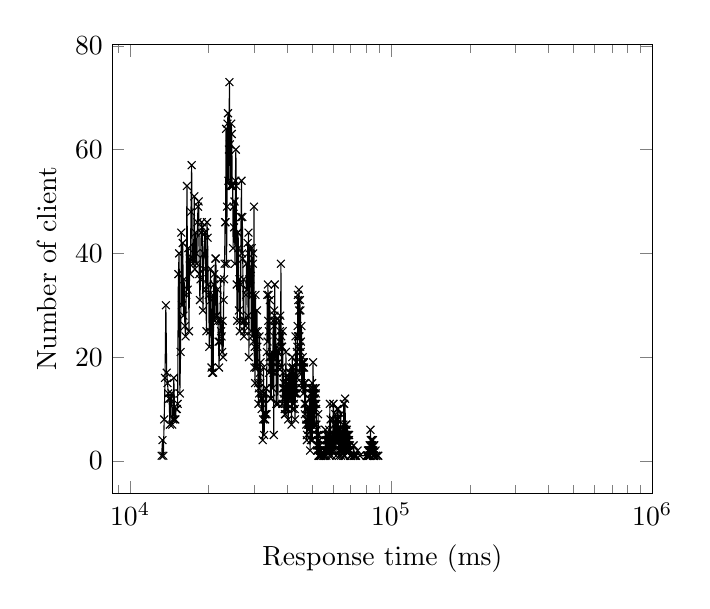
\begin{tikzpicture}
\begin{semilogxaxis}[xmin=0,xmax=1000000, ylabel=Number of client, xlabel=Response time (ms)]

\addplot[color=black, mark=x] coordinates {(13200,1)(13300,4)(13400,1)(13500,8)(13600,16)(13700,30)(13800,17)(13900,15)(14000,13)(14100,12)(14200,7)(14300,12)(14400,13)(14500,7)(14600,8)(14700,16)(14800,8)(14900,8)(15000,10)(15100,10)(15200,11)(15300,36)(15400,40)(15500,13)(15600,21)(15700,44)(15800,30)(15900,42)(16000,28)(16100,35)(16200,26)(16300,24)(16400,32)(16500,53)(16600,33)(16700,41)(16800,25)(16900,39)(17000,36)(17100,48)(17200,57)(17300,39)(17400,38)(17500,39)(17600,51)(17700,37)(17800,44)(17900,40)(18000,38)(18100,46)(18200,49)(18300,50)(18400,36)(18500,31)(18600,35)(18700,44)(18800,46)(18900,45)(19000,29)(19100,37)(19200,40)(19300,44)(19400,44)(19500,33)(19600,25)(19700,46)(19800,43)(19900,34)(20000,32)(20100,22)(20200,25)(20300,37)(20400,31)(20500,18)(20600,17)(20700,32)(20800,17)(20900,34)(21000,36)(21100,27)(21200,39)(21300,39)(21400,28)(21500,28)(21600,33)(21700,27)(21800,23)(21900,18)(22000,23)(22100,27)(22200,35)(22300,25)(22400,24)(22500,21)(22600,27)(22700,20)(22800,31)(22900,35)(23000,38)(23100,46)(23200,46)(23300,64)(23400,38)(23500,49)(23600,65)(23700,67)(23800,54)(23900,60)(24000,73)(24100,61)(24200,53)(24300,53)(24400,65)(24500,63)(24600,53)(24700,53)(24800,41)(24900,49)(25000,45)(25100,50)(25200,38)(25300,54)(25400,60)(25500,53)(25600,34)(25700,27)(25800,44)(25900,44)(26000,41)(26100,29)(26200,35)(26300,25)(26400,27)(26500,34)(26600,47)(26700,54)(26800,40)(26900,47)(27000,39)(27100,27)(27200,35)(27300,24)(27400,25)(27500,27)(27600,27)(27700,26)(27800,32)(27900,38)(28000,33)(28100,33)(28200,42)(28300,28)(28400,44)(28500,20)(28600,35)(28700,41)(28800,34)(28900,35)(29000,37)(29100,25)(29200,41)(29300,24)(29400,32)(29500,38)(29600,40)(29700,23)(29800,49)(29900,18)(30000,22)(30100,15)(30200,32)(30300,25)(30400,18)(30500,18)(30600,29)(30700,22)(30800,25)(30900,15)(31000,11)(31100,14)(31200,13)(31300,24)(31400,17)(31500,15)(31600,19)(31700,12)(31800,13)(31900,10)(32000,12)(32100,12)(32200,4)(32300,8)(32400,18)(32500,13)(32600,5)(32700,8)(32800,9)(32900,8)(33000,9)(33100,14)(33200,14)(33300,9)(33400,21)(33500,32)(33600,23)(33700,34)(33800,27)(33900,32)(34000,25)(34100,17)(34200,20)(34300,31)(34400,20)(34500,12)(34600,18)(34700,12)(34800,20)(34900,21)(35000,18)(35100,14)(35200,20)(35300,27)(35400,17)(35500,5)(35600,29)(35700,28)(35800,34)(35900,20)(36000,27)(36100,27)(36200,20)(36300,11)(36400,17)(36500,22)(36600,21)(36700,18)(36800,11)(36900,18)(37000,19)(37100,21)(37200,27)(37300,27)(37400,23)(37500,25)(37600,28)(37700,22)(37800,38)(37900,24)(38000,18)(38100,22)(38200,22)(38300,11)(38400,25)(38500,14)(38600,17)(38700,12)(38800,15)(38900,14)(39000,13)(39100,10)(39200,9)(39300,9)(39400,12)(39500,21)(39600,16)(39700,10)(39800,14)(39900,15)(40000,12)(40100,11)(40200,10)(40300,8)(40400,16)(40500,13)(40600,12)(40700,14)(40800,17)(40900,16)(41000,12)(41100,17)(41200,13)(41300,15)(41400,18)(41500,7)(41600,13)(41700,14)(41800,20)(41900,10)(42000,18)(42100,18)(42200,16)(42300,12)(42400,11)(42500,13)(42600,17)(42700,10)(42800,8)(42900,13)(43000,24)(43100,15)(43200,14)(43300,19)(43400,13)(43500,21)(43600,16)(43700,22)(43800,26)(43900,32)(44000,24)(44100,31)(44200,24)(44300,33)(44400,29)(44500,24)(44600,17)(44700,31)(44800,22)(44900,29)(45000,21)(45100,23)(45200,18)(45300,26)(45400,15)(45500,14)(45600,18)(45700,19)(45800,20)(45900,19)(46000,18)(46100,13)(46200,19)(46300,19)(46400,18)(46500,15)(46600,11)(46700,9)(46800,14)(46900,15)(47000,11)(47100,10)(47200,8)(47300,7)(47400,8)(47500,4)(47600,5)(47700,8)(47800,8)(47900,10)(48000,7)(48100,10)(48200,6)(48300,7)(48400,6)(48500,7)(48600,12)(48700,7)(48800,7)(48900,2)(49000,14)(49100,13)(49200,7)(49300,4)(49400,9)(49500,6)(49600,7)(49700,13)(49800,15)(49900,4)(50000,14)(50100,14)(50200,19)(50300,14)(50400,13)(50500,11)(50600,7)(50700,7)(50800,13)(50900,7)(51000,12)(51100,11)(51200,14)(51300,14)(51400,13)(51500,10)(51600,11)(51700,7)(51800,6)(51900,3)(52000,5)(52100,2)(52200,3)(52300,2)(52400,3)(52500,9)(52600,1)(52700,5)(52800,5)(52900,1)(53100,4)(53200,3)(53300,2)(53400,1)(53500,2)(53600,2)(53700,1)(53800,1)(53900,2)(54000,1)(54900,1)(55300,2)(55400,1)(55600,1)(55700,2)(55800,2)(55900,6)(56000,4)(56100,2)(56300,2)(56400,1)(56500,5)(56600,2)(56700,4)(56800,4)(56900,3)(57000,2)(57100,3)(57200,4)(57300,3)(57400,5)(57500,4)(57600,2)(57800,2)(57900,6)(58000,4)(58100,1)(58200,11)(58300,3)(58400,4)(58500,5)(58600,8)(58700,3)(58800,2)(58900,2)(59000,2)(59100,1)(59200,3)(59300,2)(59400,4)(59500,3)(59600,5)(59700,4)(59800,8)(59900,5)(60000,11)(60100,11)(60200,3)(60300,2)(60500,7)(60600,4)(60700,3)(60800,4)(60900,4)(61000,5)(61100,9)(61200,4)(61400,6)(61500,1)(61600,5)(61700,5)(61800,8)(61900,5)(62000,6)(62100,10)(62200,4)(62300,7)(62400,8)(62500,4)(62600,10)(62700,8)(62800,6)(62900,2)(63000,4)(63100,3)(63200,1)(63300,2)(63400,4)(63500,5)(63600,6)(63700,5)(63800,2)(63900,4)(64000,5)(64100,9)(64200,3)(64300,1)(64400,5)(64500,4)(64600,2)(64700,2)(64800,5)(64900,3)(65000,3)(65100,6)(65200,5)(65300,2)(65400,5)(65500,6)(65600,7)(65700,1)(65800,11)(65900,3)(66000,5)(66100,11)(66200,4)(66300,1)(66400,1)(66500,2)(66600,12)(66700,6)(66800,6)(66900,2)(67000,5)(67100,2)(67200,7)(67300,7)(67400,5)(67500,3)(67600,6)(67700,4)(67800,4)(67900,5)(68000,2)(68100,2)(68200,2)(68300,5)(68400,3)(68500,4)(68600,4)(68700,5)(68800,3)(68900,4)(69000,5)(69200,2)(69400,2)(69500,3)(69600,2)(69700,1)(70000,1)(70100,1)(70200,1)(71600,1)(71800,3)(72200,1)(72600,1)(73100,1)(73400,1)(74300,2)(75800,1)(80600,1)(80800,1)(81000,1)(81200,1)(81500,2)(81600,1)(81700,1)(81800,1)(81900,1)(82000,2)(82100,2)(82200,2)(82300,2)(82400,2)(82500,1)(82600,2)(82700,3)(82800,2)(82900,1)(83000,1)(83100,3)(83200,2)(83300,6)(83400,2)(83500,2)(83600,4)(83700,3)(83800,2)(83900,2)(84000,2)(84100,2)(84200,4)(84300,2)(84400,4)(84600,3)(84700,3)(85000,2)(85100,1)(85200,4)(85400,2)(85600,1)(85700,1)(85900,1)(86000,3)(86100,3)(86200,1)(87100,2)(87600,1)(88700,1)(89300,1)};
\end{semilogxaxis}
\end{tikzpicture}

\caption{Response time for count\_chain}
\label{fig:timecountchain}
\end{figure}

\begin{figure}
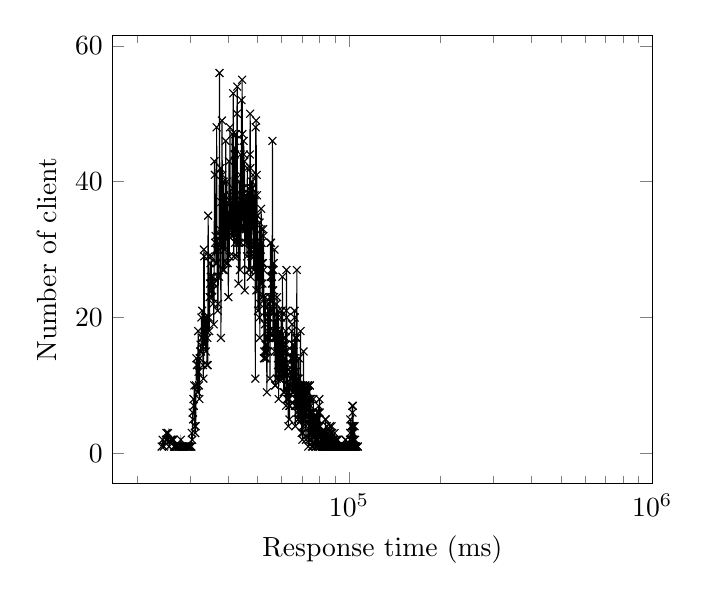
\begin{tikzpicture}
\begin{semilogxaxis}[xmin=0,xmax=1000000, ylabel=Number of client, xlabel=Response time (ms)]

\addplot[color=black, mark=x] coordinates {(24100,1)(24300,2)(24500,1)(24900,2)(25000,3)(25100,2)(25300,3)(25500,1)(25800,2)(25900,2)(26000,2)(26200,2)(26300,2)(26400,2)(26500,1)(26600,1)(26700,1)(26800,1)(26900,1)(27000,1)(27100,1)(27200,1)(27400,1)(27500,1)(27700,1)(27800,1)(27900,2)(28100,1)(28200,1)(28300,1)(28500,1)(28800,1)(28900,1)(29100,1)(29200,1)(29300,1)(29400,1)(29500,1)(29600,1)(29700,1)(29800,1)(30000,1)(30200,1)(30300,3)(30400,2)(30500,6)(30600,5)(30700,8)(30800,7)(30900,10)(31000,4)(31100,3)(31200,4)(31300,10)(31400,14)(31500,13)(31600,13)(31700,9)(31800,18)(31900,12)(32000,10)(32100,8)(32200,14)(32300,15)(32400,16)(32500,15)(32600,20)(32700,17)(32800,21)(32900,17)(33000,13)(33100,11)(33200,30)(33300,29)(33400,16)(33500,20)(33600,19)(33700,15)(33800,18)(33900,20)(34000,13)(34100,17)(34200,13)(34300,35)(34400,29)(34500,20)(34600,18)(34700,23)(34800,25)(34900,28)(35000,26)(35100,29)(35200,24)(35300,23)(35400,24)(35500,26)(35600,22)(35700,25)(35800,19)(35900,25)(36000,43)(36100,41)(36200,31)(36300,32)(36400,28)(36500,30)(36600,48)(36700,28)(36800,26)(36900,21)(37000,22)(37100,31)(37200,30)(37300,26)(37400,56)(37500,33)(37600,32)(37700,42)(37800,17)(37900,37)(38000,32)(38100,49)(38200,41)(38300,27)(38400,40)(38500,38)(38600,40)(38700,27)(38800,38)(38900,32)(39000,30)(39100,35)(39200,46)(39300,28)(39400,35)(39500,40)(39600,35)(39700,37)(39800,28)(39900,33)(40000,23)(40100,32)(40200,43)(40300,29)(40400,38)(40500,48)(40600,33)(40700,34)(40800,33)(40900,37)(41000,32)(41100,37)(41200,47)(41300,32)(41400,39)(41500,53)(41600,34)(41700,29)(41800,37)(41900,44)(42000,45)(42100,31)(42200,47)(42300,47)(42400,33)(42500,38)(42600,29)(42700,50)(42800,54)(42900,31)(43000,37)(43100,34)(43200,25)(43300,31)(43400,35)(43500,40)(43600,36)(43700,27)(43800,41)(43900,44)(44000,31)(44100,33)(44200,52)(44300,38)(44400,55)(44500,47)(44600,35)(44700,33)(44800,39)(44900,46)(45000,44)(45100,33)(45200,43)(45300,24)(45400,34)(45500,38)(45600,31)(45700,33)(45800,38)(45900,34)(46000,34)(46100,29)(46200,42)(46300,33)(46400,35)(46500,31)(46600,35)(46700,27)(46800,39)(46900,27)(47000,30)(47100,44)(47200,50)(47300,42)(47400,26)(47500,30)(47600,29)(47700,34)(47800,39)(47900,40)(48000,39)(48100,33)(48200,41)(48300,31)(48400,29)(48500,27)(48600,29)(48700,30)(48800,38)(48900,30)(49000,31)(49100,11)(49200,48)(49300,31)(49400,49)(49500,24)(49600,41)(49700,38)(49800,35)(49900,35)(50000,27)(50100,21)(50200,29)(50300,24)(50400,31)(50500,27)(50600,20)(50700,34)(50800,17)(50900,22)(51000,30)(51100,30)(51200,25)(51300,36)(51400,33)(51500,31)(51600,28)(51700,23)(51800,25)(51900,23)(52000,28)(52100,33)(52200,32)(52300,27)(52400,14)(52500,15)(52600,14)(52700,14)(52800,19)(52900,23)(53000,16)(53100,15)(53200,15)(53300,16)(53400,14)(53500,16)(53600,9)(53700,17)(53800,17)(53900,22)(54000,18)(54100,20)(54200,15)(54300,21)(54400,17)(54500,20)(54600,17)(54700,22)(54800,23)(54900,11)(55000,21)(55100,31)(55200,26)(55300,31)(55400,23)(55500,27)(55600,26)(55700,25)(55800,21)(55900,46)(56000,27)(56100,18)(56200,24)(56300,27)(56400,28)(56500,17)(56600,23)(56700,18)(56800,30)(56900,15)(57000,17)(57100,10)(57200,10)(57300,17)(57400,17)(57500,18)(57600,22)(57700,17)(57800,11)(57900,23)(58000,15)(58100,20)(58200,15)(58300,13)(58400,12)(58500,21)(58600,8)(58700,16)(58800,13)(58900,11)(59000,11)(59100,18)(59200,17)(59300,15)(59400,13)(59500,14)(59600,12)(59700,20)(59800,13)(59900,21)(60000,11)(60100,16)(60200,11)(60300,26)(60400,13)(60500,16)(60600,12)(60700,16)(60800,17)(60900,9)(61000,13)(61100,12)(61200,9)(61300,14)(61400,14)(61500,13)(61600,15)(61700,17)(61800,18)(61900,16)(62000,7)(62100,21)(62200,27)(62300,20)(62400,15)(62500,8)(62600,8)(62700,13)(62800,10)(62900,8)(63000,8)(63100,4)(63200,9)(63300,10)(63400,8)(63500,7)(63600,5)(63700,7)(63800,7)(63900,12)(64000,10)(64100,11)(64200,11)(64300,12)(64400,11)(64500,14)(64600,12)(64700,18)(64800,14)(64900,19)(65000,10)(65100,9)(65200,13)(65300,15)(65400,14)(65500,16)(65600,16)(65700,9)(65800,14)(65900,14)(66000,12)(66100,21)(66200,20)(66300,14)(66400,7)(66500,4)(66600,17)(66700,8)(66800,7)(66900,12)(67000,8)(67100,7)(67200,17)(67300,27)(67400,10)(67500,6)(67600,8)(67700,8)(67800,11)(67900,5)(68000,5)(68100,5)(68200,11)(68300,14)(68400,7)(68500,8)(68600,10)(68700,10)(68800,7)(68900,7)(69000,6)(69100,7)(69200,18)(69300,9)(69400,5)(69500,10)(69600,6)(69700,8)(69800,3)(69900,8)(70000,5)(70100,6)(70200,2)(70300,9)(70400,10)(70500,3)(70600,4)(70700,7)(70800,15)(70900,9)(71000,8)(71100,6)(71200,5)(71300,6)(71400,10)(71500,6)(71600,6)(71700,5)(71800,7)(71900,10)(72000,4)(72100,2)(72200,6)(72300,6)(72400,9)(72500,8)(72600,8)(72700,9)(72800,7)(72900,9)(73000,7)(73100,10)(73200,10)(73300,9)(73400,1)(73500,5)(73600,8)(73700,3)(73800,2)(73900,5)(74000,6)(74100,5)(74200,10)(74300,10)(74400,5)(74500,8)(74600,6)(74700,3)(74800,7)(74900,8)(75000,5)(75100,2)(75200,3)(75300,4)(75400,1)(75500,4)(75600,4)(75700,6)(75800,6)(75900,5)(76000,4)(76100,1)(76200,6)(76300,8)(76400,3)(76500,3)(76600,5)(76700,3)(76800,4)(76900,4)(77000,3)(77100,5)(77200,5)(77400,2)(77500,1)(77600,5)(77700,3)(77800,2)(78000,1)(78100,2)(78200,2)(78300,4)(78400,3)(78500,2)(78600,6)(78700,4)(78800,2)(78900,5)(79000,3)(79100,1)(79200,3)(79400,6)(79500,7)(79600,3)(79700,3)(79800,4)(79900,8)(80000,3)(80100,6)(80200,1)(80300,4)(80400,3)(80700,3)(80800,3)(80900,2)(81000,2)(81100,2)(81200,3)(81300,3)(81400,1)(81500,1)(81700,2)(81800,3)(81900,2)(82100,3)(82200,1)(82300,1)(82400,2)(82500,1)(82600,1)(82700,1)(82800,2)(82900,1)(83000,1)(83100,1)(83200,1)(83300,3)(83400,1)(83500,3)(83600,5)(83700,5)(83900,1)(84000,1)(84100,1)(84200,2)(84300,1)(84400,1)(84500,4)(84600,2)(84700,1)(84800,1)(84900,2)(85000,2)(85100,3)(85200,2)(85400,1)(85500,1)(85700,2)(85800,2)(86000,2)(86100,1)(86500,2)(86600,4)(86900,1)(87000,3)(87300,1)(87400,1)(87500,2)(87600,4)(87700,1)(87800,1)(88000,3)(88200,1)(88300,1)(88400,1)(88500,1)(88600,2)(88700,2)(88900,1)(89200,1)(89300,1)(89500,2)(89600,3)(89700,1)(90000,1)(90100,1)(90400,1)(90600,2)(90700,1)(90800,1)(91100,1)(91300,2)(91400,1)(91700,1)(91800,2)(92100,1)(92300,1)(92700,1)(92800,1)(93000,1)(93500,1)(93600,1)(93800,1)(93900,1)(94500,1)(94900,1)(95300,1)(95400,1)(95900,1)(96800,1)(97200,1)(97300,2)(97400,2)(97700,1)(98700,1)(99000,1)(99200,1)(99400,1)(99600,1)(99900,1)(100600,1)(100700,1)(100800,2)(100900,3)(101000,5)(101100,2)(101200,1)(101300,1)(101400,2)(101600,1)(101700,4)(101800,4)(101900,1)(102000,2)(102100,1)(102200,2)(102300,1)(102400,4)(102500,7)(102600,1)(102700,6)(102800,4)(102900,2)(103000,7)(103100,3)(103200,1)(103300,1)(103400,4)(103500,1)(103600,1)(103700,2)(103800,1)(104000,1)(104100,1)(104200,1)(104300,4)(104600,1)(104700,2)(104800,1)(105200,1)(105400,1)(106700,1)(107000,1)};
\end{semilogxaxis}
\end{tikzpicture}

\caption{Response time for count\_nextTick}
\label{fig:timecountnextTick}
\end{figure}

\begin{figure}
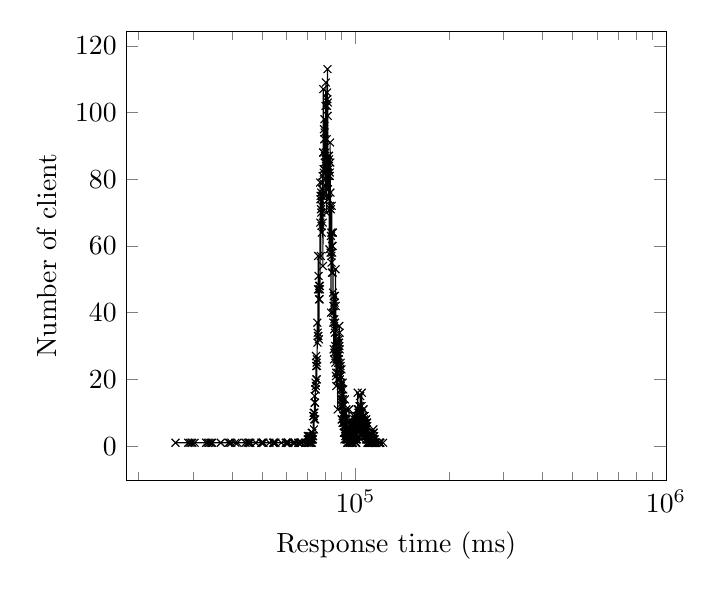
\begin{tikzpicture}
\begin{semilogxaxis}[xmin=0,xmax=1000000, ylabel=Number of client, xlabel=Response time (ms)]

\addplot[color=black, mark=x] coordinates {(26300,1)(28900,1)(29200,1)(29600,1)(29800,1)(30300,1)(33000,1)(33400,1)(33800,1)(34200,1)(34500,1)(36800,1)(39000,1)(39300,1)(39800,1)(41000,1)(41600,1)(44200,1)(44900,1)(45300,1)(45500,1)(45800,1)(47700,1)(49700,1)(50000,1)(50300,1)(50500,1)(52800,1)(54300,1)(54500,1)(54700,1)(55200,1)(57700,1)(59600,1)(59900,1)(60200,1)(60500,1)(60700,1)(62900,1)(63200,1)(63700,1)(65300,1)(65600,1)(66500,1)(66800,1)(67000,1)(68900,1)(69700,1)(70100,2)(70200,3)(70300,2)(70400,3)(70500,1)(70600,2)(70700,2)(70900,1)(71000,3)(71100,2)(71200,2)(71300,3)(71400,1)(71600,2)(71700,3)(71800,1)(71900,1)(72000,2)(72100,2)(72200,4)(72300,1)(72400,2)(72500,2)(72600,4)(72700,3)(72800,3)(72900,2)(73000,3)(73100,9)(73200,9)(73300,10)(73400,9)(73500,5)(73600,8)(73700,10)(73800,15)(73900,13)(74000,13)(74100,8)(74200,17)(74300,19)(74400,17)(74500,18)(74600,27)(74700,24)(74800,20)(74900,25)(75000,20)(75100,26)(75200,24)(75300,37)(75400,31)(75500,34)(75600,33)(75700,47)(75800,57)(75900,33)(76000,51)(76100,47)(76200,32)(76300,44)(76400,48)(76500,48)(76600,44)(76700,48)(76800,47)(76900,79)(77000,67)(77100,74)(77200,75)(77300,57)(77400,71)(77500,76)(77600,70)(77700,66)(77800,64)(77900,72)(78000,75)(78100,77)(78200,79)(78300,81)(78400,67)(78500,54)(78600,88)(78700,107)(78800,88)(78900,83)(79000,82)(79100,95)(79200,83)(79300,92)(79400,98)(79500,94)(79600,85)(79700,87)(79800,76)(79900,87)(80000,102)(80100,88)(80200,109)(80300,86)(80400,75)(80500,83)(80600,70)(80700,92)(80800,83)(80900,102)(81000,106)(81100,104)(81200,113)(81300,99)(81400,103)(81500,77)(81600,84)(81700,81)(81800,74)(81900,83)(82000,87)(82100,87)(82200,86)(82300,59)(82400,81)(82500,81)(82600,82)(82700,72)(82800,91)(82900,85)(83000,76)(83100,58)(83200,71)(83300,63)(83400,40)(83500,64)(83600,57)(83700,55)(83800,72)(83900,52)(84000,60)(84100,58)(84200,64)(84300,60)(84400,52)(84500,64)(84600,46)(84700,40)(84800,37)(84900,42)(85000,29)(85100,45)(85200,26)(85300,35)(85400,38)(85500,28)(85600,43)(85700,45)(85800,34)(85900,37)(86000,30)(86100,25)(86200,53)(86300,42)(86400,29)(86500,21)(86600,22)(86700,18)(86800,26)(86900,29)(87000,32)(87100,28)(87200,31)(87300,26)(87400,27)(87500,22)(87600,11)(87700,20)(87800,27)(87900,25)(88000,25)(88100,28)(88200,31)(88300,26)(88400,32)(88500,31)(88600,36)(88700,30)(88800,34)(88900,29)(89000,20)(89100,23)(89200,21)(89300,21)(89400,24)(89500,25)(89600,18)(89700,17)(89800,14)(89900,19)(90000,17)(90100,23)(90200,8)(90300,12)(90400,15)(90500,8)(90600,13)(90700,14)(90800,7)(90900,19)(91000,14)(91100,12)(91200,9)(91300,17)(91400,7)(91500,10)(91600,6)(91700,4)(91800,7)(91900,4)(92000,6)(92100,2)(92200,10)(92300,10)(92400,14)(92500,8)(92600,3)(92700,5)(92800,4)(92900,7)(93000,5)(93100,2)(93200,4)(93300,8)(93400,11)(93500,3)(93600,2)(93700,2)(93800,5)(93900,3)(94000,1)(94100,5)(94200,2)(94300,3)(94400,2)(94500,1)(94600,4)(94700,3)(94800,5)(94900,2)(95000,3)(95100,5)(95200,7)(95300,11)(95400,7)(95500,1)(95600,5)(95700,3)(95800,2)(96000,1)(96200,3)(96300,2)(96400,3)(96500,2)(96600,4)(96700,4)(96800,2)(97000,1)(97100,2)(97300,4)(97400,1)(97500,1)(97600,3)(97700,2)(97800,1)(97900,4)(98000,1)(98100,4)(98200,2)(98300,2)(98400,7)(98500,2)(98600,2)(98700,2)(98800,7)(98900,9)(99000,8)(99100,6)(99200,5)(99300,7)(99400,4)(99500,3)(99600,4)(99700,7)(99800,6)(99900,3)(100000,2)(100100,1)(100200,8)(100300,2)(100400,5)(100500,1)(100600,9)(100700,6)(100800,6)(100900,5)(101000,9)(101100,2)(101200,7)(101300,8)(101400,8)(101500,11)(101600,16)(101700,4)(101800,6)(101900,7)(102000,11)(102100,10)(102200,11)(102300,7)(102400,9)(102500,8)(102600,10)(102700,6)(102800,6)(102900,10)(103000,12)(103100,7)(103200,12)(103300,6)(103400,10)(103500,15)(103600,9)(103700,7)(103800,7)(103900,6)(104000,10)(104100,2)(104200,8)(104300,4)(104400,3)(104500,7)(104600,12)(104700,16)(104800,6)(104900,7)(105000,5)(105100,5)(105200,6)(105300,4)(105400,7)(105500,6)(105600,7)(105700,9)(105800,9)(105900,6)(106000,11)(106100,11)(106200,7)(106300,5)(106400,8)(106500,9)(106600,7)(106700,5)(106800,4)(106900,9)(107000,3)(107100,3)(107200,5)(107300,5)(107400,5)(107500,4)(107700,6)(107800,3)(107900,4)(108000,8)(108100,2)(108200,8)(108300,5)(108400,3)(108500,3)(108600,7)(108700,7)(108800,2)(108900,7)(109000,3)(109100,6)(109200,1)(109300,2)(109500,4)(109600,2)(109800,3)(109900,1)(110100,2)(110200,3)(110300,1)(110400,3)(110500,1)(110600,2)(110800,3)(110900,1)(111100,1)(111200,1)(111600,2)(111900,2)(112200,1)(112400,1)(112500,1)(112600,3)(112700,2)(112800,2)(113000,2)(113100,1)(113200,2)(113400,1)(113600,1)(113700,2)(113800,2)(114000,1)(114100,5)(114200,4)(114300,4)(114700,2)(114800,3)(115000,1)(115200,2)(115300,1)(115400,1)(115500,1)(115700,1)(115800,1)(116200,1)(116600,1)(119000,1)(119300,1)(119600,1)(119900,1)(120200,1)(122600,1)};
\end{semilogxaxis}
\end{tikzpicture}

\caption{Response time for count\_setTimeout}
\label{fig:timecountsetTimeout}
\end{figure}


We can see that the use of fluxions, from our implementation of the fluxionnal execution model increases the average response time of about 50\%, as the \textbf{Fluxionnal-NoSetTimeout} implementation aberage response time show from the \textbf{Basic} implementation.
However, the instruction \texttt{SetTimeout}, used in the original Fluxionnal execution model, increases the average response time of this implementation of about 360\%.



\TODO{}
Although, using a fluxionnal approach is a way to build an efficient distributed system we consider that the most important part of our work is to enable code transformation from a standard basic web approach to a flow of fluxions.
We show now the main code transformation we propose.